% ==================================================
% Perception System 
% Author: Lester James V. Miranda
% ==================================================

\documentclass[preview, convert={outfile=\jobname-out.png,density=300}]{standalone}

\usepackage{tikz}
\usepackage{color}
\usepackage{subfig}
\usepackage{ifthen}
\usepackage{graphicx}
\usepackage{fontawesome}

\renewcommand\familydefault{\sfdefault}

\usetikzlibrary{
    matrix,
    shapes,
    fit,
    arrows,
    positioning,
    calc,
    backgrounds,
    shadows.blur,
    shapes.geometric,
}


% taken from manual
\makeatletter
\pgfdeclareshape{document}{
\inheritsavedanchors[from=rectangle] % this is nearly a rectangle
\inheritanchorborder[from=rectangle]
\inheritanchor[from=rectangle]{center}
\inheritanchor[from=rectangle]{north}
\inheritanchor[from=rectangle]{south}
\inheritanchor[from=rectangle]{west}
\inheritanchor[from=rectangle]{east}
% ... and possibly more
\backgroundpath{% this is new
% store lower right in xa/ya and upper right in xb/yb
\southwest \pgf@xa=\pgf@x \pgf@ya=\pgf@y
\northeast \pgf@xb=\pgf@x \pgf@yb=\pgf@y
% compute corner of ‘‘flipped page’’
\pgf@xc=\pgf@xb \advance\pgf@xc by-10pt % this should be a parameter
\pgf@yc=\pgf@yb \advance\pgf@yc by-10pt
% construct main path
\pgfpathmoveto{\pgfpoint{\pgf@xa}{\pgf@ya}}
\pgfpathlineto{\pgfpoint{\pgf@xa}{\pgf@yb}}
\pgfpathlineto{\pgfpoint{\pgf@xc}{\pgf@yb}}
\pgfpathlineto{\pgfpoint{\pgf@xb}{\pgf@yc}}
\pgfpathlineto{\pgfpoint{\pgf@xb}{\pgf@ya}}
\pgfpathclose
% add little corner
\pgfpathmoveto{\pgfpoint{\pgf@xc}{\pgf@yb}}
\pgfpathlineto{\pgfpoint{\pgf@xc}{\pgf@yc}}
\pgfpathlineto{\pgfpoint{\pgf@xb}{\pgf@yc}}
\pgfpathlineto{\pgfpoint{\pgf@xc}{\pgf@yc}}
}
}
\makeatother


\begin{document}
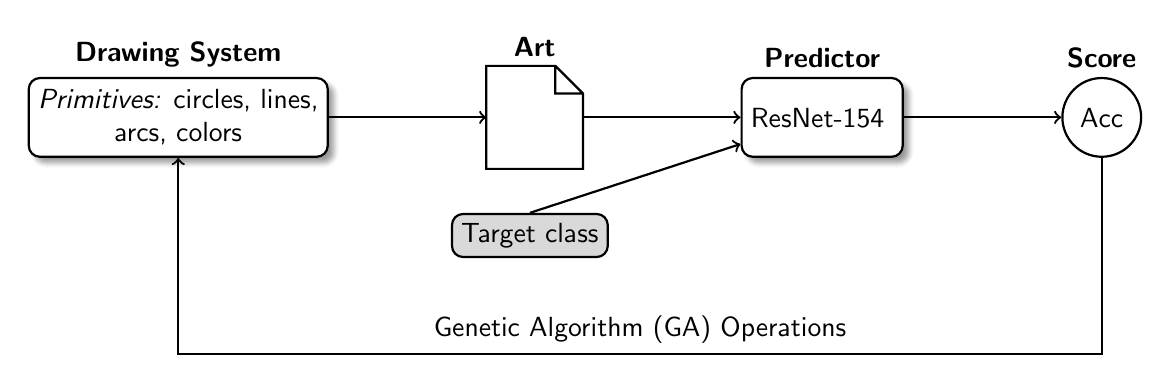
\begin{tikzpicture}[
    node distance= 2cm,
    module/.style={draw, thick, rounded corners, text=black, align=center,
                minimum width=2cm,minimum height=1cm,fill=white, 
                blur shadow={shadow blur steps=5}},
    file/.style={draw, shape=document, minimum width=1.2cm, minimum
                height=1.28cm, thick, fill=white}
]

% Drawing System
\node[module, label={\bfseries Drawing System}] at (0,0) (Primitives) {
    \textit{Primitives:} circles, lines,\\ arcs, colors
};

% Output image
\node[file, label={\bfseries Art}] (OutputImage) [right=of Primitives] {};

% Target class
\node[rounded corners, draw, thick, fill=black!15, align=center] (Target) [right=of
Primitives, yshift=-1.5cm, xshift=-0.45cm] {Target class};

% Predictor
\node[module, label={\bfseries Predictor}] [right=of OutputImage] (Predictor) {
    ResNet-154
};

% Score
\node[circle, draw, thick, minimum width=1cm, label={\bfseries Score}] [right=of Predictor]
(Score) {Acc};

% Draw lines
\draw[->, thick] (Primitives) -- (OutputImage) {};
\draw[->, thick] (OutputImage) -- (Predictor) {};
\draw[->, thick] (Target.north) -- (Predictor) {};
\draw[->, thick] (Predictor) -- (Score) {};
\draw[->, thick] (Score) |- ++(0,-3cm) -| (Primitives) 
    node[pos=0.25, above, align=center] {Genetic Algorithm (GA) Operations};


\end{tikzpicture}
\end{document}

